\chapter{Case study}
\label{chap:case_study}

\section{Overview}

The goal of our case study introduced in this chapter is to show the application and working of our hierarchical runtime verification framework. The motivation of this study is the related report from 2014 \citep{tdk2014}, where the goal was a distributed, model based security logic. The work of [1] focused on the model driven development of a safety logic and its application in the Model Railway Project. Our work builds on the hardware and software of [1] and extends it with the runtime verification of:
\begin{itemize}
	\item The working of the safety logic in the embedded controllers.
	\item The correctness of the overall system.
\end{itemize}

\begin{figure}[h]
	\centering
	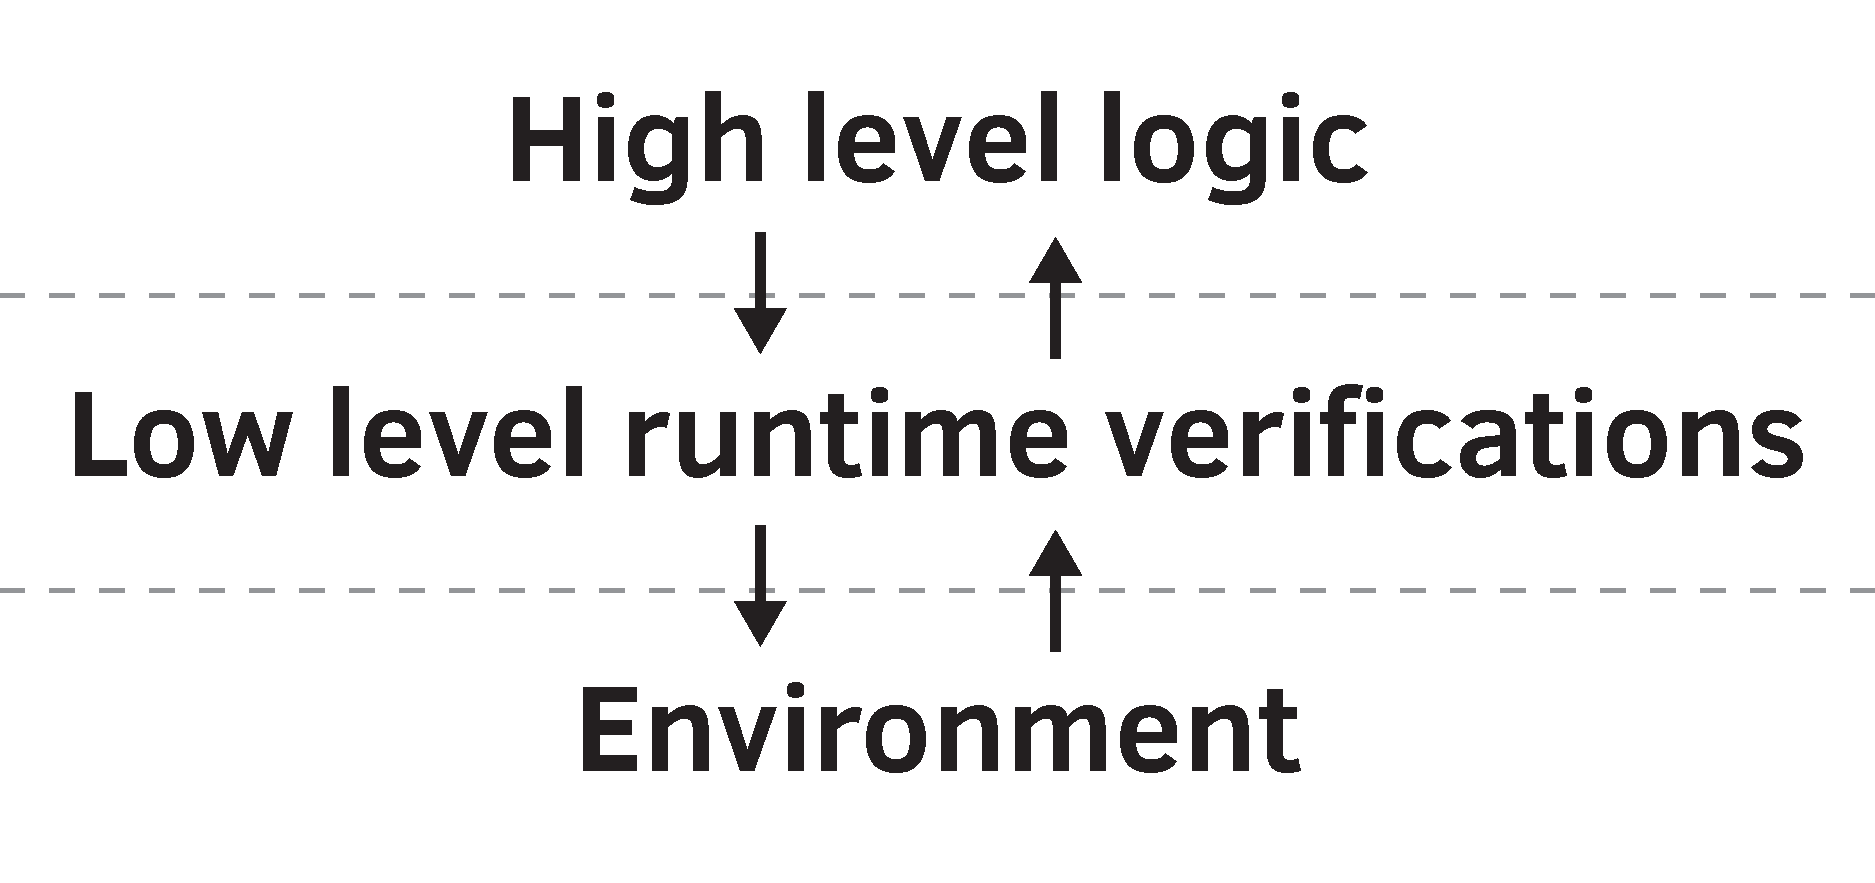
\includegraphics[width=0.5\linewidth]{include/figures/chapter_6/overview_1}
	\caption{Overview of the hierarchical runtime verification system}
	\label{fig:case_study:fov}
\end{figure}

In this section at first we overview those concepts of the Model Railway Project which are important from our point of view. Then the extended runtime verification architecture is introduced both the hardware and software components.

It's important to notice that our solution is not tailored to this special problem but it is a general approach for any critical system.

\section{Concept}

Our main goal with this study is to develop a method which can integrate multiple safety logic into a global runtime verification, increasing the reliability of the complete system.

\begin{figure}[h]
	\centering
	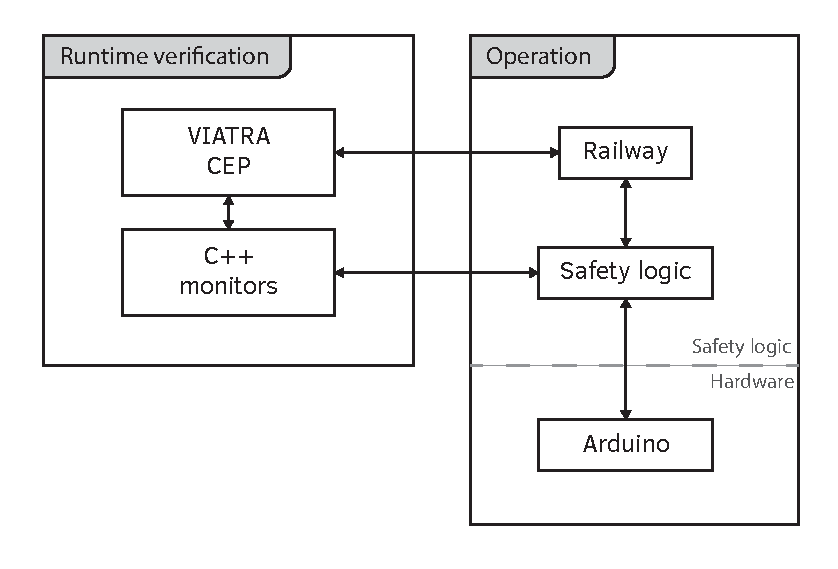
\includegraphics[width=0.75\linewidth]{include/figures/chapter_6/concept_1}
	\caption{Associations between operation, and runtime verification components}
	\label{fig:case_study:concept_component}
\end{figure}

\cref{fig:case_study:concept_component} shows the main relation between the operation, and runtime verification domain. With component level verification -- in out case with embedded monitors -- we can verify each component runtime state. The system level verification observes the overall state of the system. If any of the components reports failure, we can make a decision based on the remaining components abilities to support the system verification. If we can provide safety despite component failures, the system can continue operation.

\begin{figure}[h]
	\centering
	\includegraphics[width=0.75\linewidth]{include/figures/chapter_6/concept_2}
	\caption{Sensor, and monitor relation}
	\label{fig:case_study:concept_communication}
\end{figure}

In our case (\cref{fig:case_study:concept_communication}), there are embedded components, and one system level component.

\section{System level verification with computer vision}

\subsection{Hardware}
\label{sec:case_study:hardware}

In case of a computer vision (\textls{CV}) based approach, it is critical to choose the appropriate hardware. We had two parameters in the selection of the camera: height above the board, and \textls{FOV}. The camera we used have these parameters:
\begin{itemize}
	\item Resolution: 1920x1080
	\item Horitontal FOV: \ang{120}
\end{itemize}

The camera have an installation height of $120$\si{\centi\meter}. This is a perfect value for using the case study in any room, and not suffer serious perspective distortions.

\subsection{OpenCV}

One key point of this study from the technological viewpoint is computer vision. It is a new extension of the hardware, which allows us to monitor the board with fairly big precision and reliability, if the correct techniques and materials are used.

We needed a fast, reliable, efficient library to use with the camera, and develop the detection algorithm. Our choice was the OpenCV\footnote{\url{http://opencv.org/}} library, which is an industry leading, open source computer vision library. It implements various algorithms with effective implementation e.g. using the latest streaming vector instruction sets. The main programming language -- and what we used -- is \textls{C++}, but it has many binding to other popular languages like Java, and Python.

\subsection{Marker design}

One of the steps of the \textls{CV} implementation was the design of the markers, which should provide an easy detection, and identification of the marked objects.

The first step was to consider the usage of an external library, named \textls{ArUco}\footnote{\url{http://www.uco.es/investiga/grupos/ava/node/26}}. This library provides the generation and detection library of markers. The problem with the library was the lack of tolerance in quality, and motion blur. Because these negative properties of the existing libraries, we implemented a marker detection algorithm for our needs.

After the implementation was in our hands, we could make markers which suits our needs. The chosen size of the marker was the size of the model railroad car as it will provide the proper accuracy.

As explained in \cref{fig:case_study:opencv_math}, circular patterns are well suited for these applications. The final design consists two detection circle, and a color circle for identification between the detection circles (\cref{fig:case_study:final_marker}).

\begin{figure}[h]
	\centering
	\includegraphics[width=0.5\linewidth]{include/figures/chapter_6/opencv_finalmarker}
	\caption{The final marker design}
	\label{fig:case_study:final_marker} 
\end{figure}

\subsection{Mathematical solution for marker detection}
\label{fig:case_study:opencv_math}

%According to the various conditions, the marker detection has to be robust.

According to the various condition in lighting, and used materials, the marker detection has to be robust.

This problem, and the fact that these markers have perspective distortion when they are near to the visible region of the camera motived us to develop a processing technique coming from signal processing.

This method is the commonly used technique of transforming and processing a signal -- in our case a picture -- in frequency domain.

\subsubsection{Convolution method}
\label{sec:case_study:convolution}

Our method is based on the convolution of two bitmap images, one from the camera, and one generated pattern.

The theorem says, we can multiply two spectrums, and apply an inverse Fourier transform to get the convoluted image. If one image is the pattern, the other image is the raw\footnote{In our application raw (or raw image) means the unprocessed image from the camera}, applying the convolution results in an image where every pixel represents a value how much the two spectrums match.

\subsubsection{Pattern bitmap properties}

The prerequisite of the pattern is the pattern must be the same size of the raw image, and the raw image must be a grayscale image.

The pattern itself needs to be generated with values according to the shape we would like to match (\cref{fig:case_study:convoluter_image}). The raw pixels are multiplied by this value. The meaning of these values in the bitmap are the following: 
\begin{itemize}
	\item \bm{$value = 0$}: Doesn't affect the match.
	\item \bm{$value > 0$}: The multiplied raw pixel summed positively to the result of the convolution.
	\item \bm{$value < 0$}: The multiplied raw pixel summed negatively to the result of the convolution.
\end{itemize}

\begin{figure}[h]
	\centering
	
\includegraphics[valign=c,width=.65\linewidth]{include/figures/chapter_6/math_2}
	\rlap{\hspace{5pt}\begin{tabular}[c]{@{}cr@{}}
		\toprule
		\tikz \node [minimum width=1ex,minimum height=1ex,fill=black] {}; & $-1$ \\
		\tikz \node [minimum width=1ex,minimum height=1ex,fill=patternGreen] {}; & $0$ \\
		\tikz \node [minimum width=1ex,minimum height=1ex,fill=white,draw=black] {}; & $1$ \\
		\bottomrule
	\end{tabular}}
	\caption{Pattern bitmap placement and value example}
	\label{fig:case_study:convoluter_image}
\end{figure}

\subsection{Software}

With the OpenCV library, we implemented a processing pipeline which can process the live video feed from the camera. We forward this data to the high level safety logic, which can decide the following actions. The \cref{table:case_study:pipeline} shows all the essential steps in the processing pipeline of the computer vision.

We used GPU acceleration trough pipeline stage 1--4. The acceleration is implemented by OpenCV, and can be used with CUDA capable NVidia video accelerators.

\begin{table}[p]
	\centering
	\setlength{\fboxsep}{0pt}
	\setlength{\fboxrule}{1pt}
	\begin{tabularx}{\textwidth}{cm{5cm}X}
		\toprule
		Stage \# & Description & Example images  \\
		\midrule
		1 & Loading an image from the camera &\fbox{\includegraphics[valign=c,width=\linewidth]{include/figures/chapter_6/stages/s1}} \\[10.5ex]
		2 & Convert the image to grayscale & \fbox{\includegraphics[valign=c,width=\linewidth]{include/figures/chapter_6/stages/s2}} \\[10.5ex]
		3 & Convolve the image with the pattern & \fbox{\includegraphics[valign=c,width=\linewidth]{include/figures/chapter_6/stages/s3}} \\[8.5ex]
	\end{tabularx}
	\begin{tabularx}{\textwidth}{cX}
		\toprule
		Stage \# & Description  \\
		\midrule
		4 & Applying a threshold to filter the brightest spots \\
		5 & Finding the contours of the enclosed shapes \\
		6 & Calculating the center point of the contours \\
		7 & Find possible markers by distance \\
		8 & ID the marker by the center \\
		\bottomrule
	\end{tabularx}
	\caption{Computer vision processing pipeline}
	\label{table:case_study:pipeline}
\end{table}

\section{Summary}
With this implementation, we can follow the system real-time, providing the high-level logic another independent source of information. This can lead to a more robust system with added redundancy.

\newpage
\section{Model railroad}
In this section we briefly overview the railroad and the controlling hardware.

\subsection{Overview}

\noindent The model railroad (\cref{fig:case_study:total_map}) contains the following hardware elements:
\begin{itemize}
	\item 15 powerable section
	\item 6 railroad switch
	\item 6 Arduino controllers for each switch
	\item 3 remotely controllable train
\end{itemize}

\begin{figure}[h]
	\centering
	\includegraphics[width=0.8\linewidth]{include/figures/chapter_6/total_view_1}
	\caption{The railroad network with section IDs}
	\label{fig:case_study:total_map}
\end{figure}

\subsection{Hardware}
The core of the railroad hardware are the Arduino microcontrollers which collects information, and control the sections. For every railroad switch there is an associated controller which can control the power of the sections nearby with the slave units connected to it (\cref{fig:case_study:master_slave}).

\begin{figure}[h]
	\centering
	\includegraphics[width=0.8\linewidth]{include/figures/chapter_6/railroad_ms}
	\caption{Master-slave associations}
	\label{fig:case_study:master_slave}
\end{figure}

\section{Metamodel design}
In this section we proceed through the design of the physical to logical mapping. We operate our safety on this logical model, so it is very important to map all the details of the physical world we need correctly in this model.

\subsection{Physical elements}
The only external source of information is the computer vision. The CV forward a train ID (determined by marker color) and position (x, y coordinates) to the model, and we must discretize these informations to make it searchable by our safety logic for hazardous events.

Let us take a look on the main components of the physical system, and what challenges we face:
\begin{itemize}
	\item \textbf{Section}: Either a rail, or railroad switch. Every section has a distinctive identifier.
	\item \textbf{Rail}: The rail is a variable length curve. The main challenge is the determination of the next section. Only the rail can be powered down, so our safety logic must act, when the train is on a rail.
	\item \textbf{Railroad switch}: The switch is a region, where we know the entry and outgoing section by its setting. The switch is always powered, so we cannot affect the train on the switch. There are some basic concept:
	\begin{itemize}
		\item A switch consists of three rails: the central rail, and two rails we can choose of, a divergent and a straight rail.
		\item \textbf{Straight rail}: The straight rail follows the central rail without a curve.
		\item \textbf{Divergent rail}: The divergent rail moves away from the imaginary line of the central rail.
	\end{itemize}
\end{itemize}

\begin{figure}[h]
	\centering
	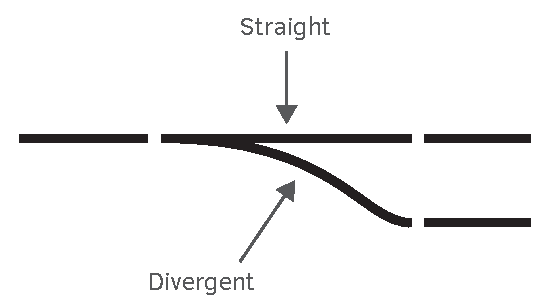
\includegraphics[width=0.5\linewidth]{include/figures/chapter_6/metamodel_switch_basics}
	\caption{Switch straight, and divergent rails}
	\label{fig:case_study:metamodel_switch_basics}
\end{figure}

\begin{figure}[h]
	\centering
	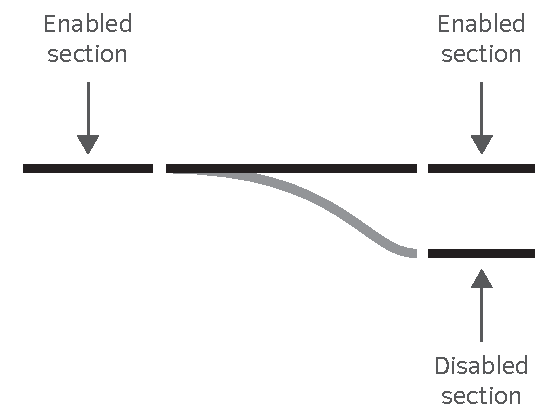
\includegraphics[width=0.5\linewidth]{include/figures/chapter_6/metamodel_switch_endi}
	\caption{Enabled-disabled section explanation}
	\label{fig:case_study:metamodel_switch_endi}
\end{figure}

\subsection{Logical breakdown of physical elements}
\label{sec:case_study:logical_breakdown}
After we designated the physical elements, and their properties, we started to build a logical concept what are our model elements, and what are the connections between them.

We will follow a bottom-up structure because it helps the graph search (\cref{sec:case_study:pattern_building}), and review the main components of the logical elements.

\begin{enumerate}
	\item \textbf{SectionModel}: The root of the board model. It is separated from trains because this root element is persisted, and loaded at every start of the application, while the \emph{TrainModel} is dynamic.
	\begin{enumerate}
		\item \textbf{Configuration}: Contains the enabled \emph{groups} of the switch.
		\item \textbf{SwitchSetting}: Contains a straight, and divergent \emph{configuration}.
		\item \label{itm:case_study:region} \textbf{Region}: The atomic abstract element of our model, the \emph{region} is the smallest unit of measurement.
		\item \textbf{SectionRegion}: Specialized region, which is a part of a \emph{powerable group}. Only powerable section can stop a train. 
		\item \textbf{RailRegion}: Specialized region. Because we did not intrested in the position inside the switch, we declare the entire area of the switch as one region.
		\item \label{itm:case_study:group} \textbf{Group}: The group is a collection of regions.
		\item \textbf{PowerableGroup}: A collection of \emph{regions} which can shutted of. The equivalent to the rail concept of the modelled study.
		\item \textbf{SwitchGroup}: A group of exacty one \emph{SwichRegion}. Have a reference to a \emph{Configuration}, describing the current switch settings.
	\end{enumerate}
	\item \textbf{TrainModel}: The root of all train elements.
	\begin{enumerate}
		\item \textbf{Train}: The train representation with an unique ID, the current and previous region (\cref{itm:case_study:region}), and the next group (\cref{itm:case_study:group}) determined by the current, and previous region.
	\end{enumerate}
\end{enumerate}

\begin{figure}[p]
	\centering
	\includegraphics[width=\linewidth]{include/figures/chapter_6/sectionmodel}
	\caption{The metamodel of the \emph{Model Railway Project} model} 
	\label{fig:case_study:model}
\end{figure}

\subsection{Introducing to Eclipse Modeling Framework}
\begin{quotation}
	``The EMF project is a modeling framework and code generation facility for building tools and other applications based on a structured data model. From a model specification described in XMI, EMF provides tools and runtime support to produce a set of Java classes for the model, along with a set of adapter classes that enable viewing and command-based editing of the model, and a basic editor.'' \cite{EMF}
\end{quotation}

We used the EMF tool to create the metamodel of the railway. The main reason for this modeling tool is the dependency to IncQuery, but other reasons motivated the use of it:
\begin{itemize}
	\item Besides the POJO\footnote{Plain Old Java Object}, EMF can generate an Eclipse based editor for the model, where we can add/remove/edit all the elements, and their properties easily. TODO The editor ensure the model.
	\item The framework ensure all the references are valid, by updating them automatically.
	\item We can make opposite edges, which are forward/backward references across two object. The framework will maintain these references e.g. we assign object A to object B, if they have a bidirectional reference between them, the EMF will automatically update the other side of the reference, in our case the reference from A to B.
\end{itemize}

\subsection{Building the EMF model}

After the conceptual design of the model, we started the design of the EMF model.

It's important while building the EMF model that every element must be a part of exactly one containament tree. If an element is not in a tree or it is in multiple tree, it causes failure while serializing. In \cref{sec:case_study:logical_breakdown} the \emph{TrainModel} and \emph{SectionModel} represents the root of the model.

\subsection{Introducing the IncQuery}

\begin{quotation}
	EMF-IncQuery is a framework for defining declarative graph queries over EMF models, and executing them efficiently without manual coding in an imperative programming language such as Java.

	With EMF-IncQuery, you can:
	\begin{itemize}
		\item Define model queries using a high level yet powerful query language (supported by state-of-the-art Xtext-based development tools)
		\item Execute the queries efficiently and incrementally, with proven scalability for complex queries over large instance models
		\item Integrate queries into your applications using essential feature APIs including IncQuery Viewers, Databinding, Validation and Query-based derived features with notifications.
	\end{itemize}
\end{quotation}

The motivation of using IncQuery can be found in the nature of our problem. The railway can be depicted as a graph, and we can describe hazardous patterns e.g. two trains next section is the opposite trains next section. These scenarios can be declaratively described by IncQuery patterns, reducing the possibility of a coding failure. The other advantage of using the IncQuery framework is scalability. The IncQuery framework -- as its name suggest: incremental query -- is a fast, caching engine based on the RETE algorithm. This framework can follow changes in a very large environment. 

\subsection{Building the IncQuery patterns}
\label{sec:case_study:pattern_building}

Let us examine the patterns providing the essential filtering of hazardous patterns in the environment.
\\[1ex]

\begin{lstlisting}[caption={Collision detection},label=lst:case_study:train_will_collide]
pattern trainAtNextGroup(t1: Train) {
	Train.nextGroup(t1, ng);
	
	Train(t2);
	t1 != t2;
	
	Train.currentlyOn(t2, co);
	Group.regions(ng, co);
}
\end{lstlisting}

\cref{lst:case_study:train_will_collide} shows an IncQuery example. This pattern matches \verb+t1+ which next group -- if not null, e.g. the train is stationary -- has a different train on it (\verb+t2+).

This example clearly presents the advantage of this declarative expression. With the right metamodel we designed an incrementially executed scalable pattern only with 5 lines of code.
\\[1ex]

\begin{lstlisting}[caption={Collision detection},label=lst:case_study:train_at_next_powerable]
pattern trainAtNextPowerable(t1: Train) {
	Train.nextGroup(t1, ng);
	Train.currentlyOn(t1, t1co);
	
	SwitchGroup(ng);
	SwitchGroup.configuration.enabled(ng, enabled);
	enabled != t1co;
	
	Train(t2);
	t1 != t2;
	Train.currentlyOn(t2, t2co);
	Group.regions(t2g, t2co);
	
	enabled == t2g;
}
\end{lstlisting}

\cref{lst:case_study:train_at_next_powerable} is a pattern for finding the next powerable group in the direction of. We must do that because the property of the switch group: a train cannot stop on that. With \cref{lst:case_study:train_will_collide} we can filter the hazards in the next group, but if we are on a switch, the train cannot be stopped; the trains might crash. This pattern is specialized in case of a train going towards a switch. We are virtually going through it, and examine the other side. If any train is present, the pattern will match, switching the power off the section.
\\[1ex]

\begin{lstlisting}[caption={Collision detection},label=lst:case_study:train_at_next_powerable]
pattern trainFromDisabled(t: Train) {
	SwitchGroup(sg);
	SwitchGroup.regions(sg, region);
	SwitchGroup.configuration.enabled(sg, enabled);
	region != enabled;
	
	Train.currentlyOn(t, region);
	Train.nextGroup(t, sg);
}
\end{lstlisting}

\cref{lst:case_study:train_at_next_powerable} is a pattern for finding the next powerable group in the direction of. We must do that because the property of the switch group: a train cannot stop on that. With \cref{lst:case_study:train_will_collide} we can filter the hazards in the next group, but if we are on a switch, the train cannot be stopped; the trains might crash. This pattern is specialized in case of a train going towards a switch. We are virtually going through it, and examine the other side. If any train is present, the pattern will match, switching the power off the section.

\section{Summary}

The Train Benchmark\cite{TrainBenchmark} shows a similar railroad approach application with IncQuery based pattern matching. Their benchmark showed IncQuery can match pattern on a similar railroad model with element sizes over 80 million under 100 milliseconds after initial caching.